\chapter{Diseño y Especificación}
\label{chap:diseno}


\section{Introducción}
\gotrev{Última revisión: 25/06/12}

Este capítulo se centrará en el análisis y especificación realizados sobre el sistema, previos a la implementación. Para ello, se detallará la captura de requisitos que definen la funcionalidad del sistema, para luego analizar con detalle los algoritmos diseñados para llevar a cabo las dos funciones más importantes de la aplicación: el análisis de imágenes y la composición de piezas musicales.

\section{Usuarios}
\label{sec:users}
\gotrev{Última revisión: 20/06/12}\\
	Los usuarios que se tienen en cuenta para delimitar los requisitos son:
	
	\begin{itemize}
		\item Usuario: Individuos con un conocimiento mínimo o nulo sobre música y ofimática que hayan leído o se les haya explicado el funcionamiento de la aplicación. Pueden requerir cierto período de entrenamiento para acostumbrarse a las distintas opciones y funciones que ofrece la aplicación.
		\item Desarrollador: Individuos con un conocimiento amplio de programación y con conocimiento básico o avanzado de música. Podrán expandir la aplicación de forma sencilla añadiendo nuevos algoritmos de composición.
		
	\end{itemize}


\section{Requisitos}
\label{sec:requisitos}
\gotrev{Última revisión: 20/06/12}\\
	Esta sección describirá las funcionalidades del sistema: su comportamiento esperado así como sus restricciones de rendimiento y capacidad. Aunque el proyecto que nos ocupa ha sido desarrollado sin ningún cliente específico, se han elaborado requisitos basados en nuestra visión de la aplicación como conjunto, de forma que tanto la planificación como el desarrollo se pudieran abordar más fácilmente.\\
	
	Una vez determinandos qué usuarios harán uso de la aplicación, se procederá a determinar cuáles son los requisitos funcionales y los no funcionales.
	
	\subsection{Requisitos funcionales}
	
	En el caso de la interfaz gráfica y la estructura general de la aplicación. La interfaz deberá ser capaz de:
	
	 \begin{itemize}
		 \item Lanzar tanto el módulo de análisis como el módulo de composición de forma independiente.
		 \item Interpretar archivos de imagen del formato .png y mostrarlos por pantalla.
		 \item Interpretar archivos de audio del formato .wav y permitir funciones básicas de reproducción sobre los mismos.
		 \item Generar un archivo de configuración interpretable tanto por la aplicación de análisis y composición a partir de los parámetros de entrada establecidos por el usuario.
		 \item Mostrar la partitura de la música compuesta tras haber sido generada mediante un programa externo o por sí misma.
		 \item Mostrar la salida del proceso de análisis de imagen (mediante un programa externo o por sí misma), en forma de polígonos con color plano distribuidos unos dentro de otros.
		 \item Controlar posibles errores cometidos por el usuario, surgidos al tocar parámetros no disponibles para la configuración seleccionada, a su vez deberá de limitar las acciones del usuario a la hora de modificar dichos parámetros según las configuraciones elegidas.
		 \item Prestar la opción de detener módulos lanzados para que el usuario pueda pararlos, si estos no han acabado aún.
	 \end{itemize}
	 
 
 En el caso del módulo de análisis de imágenes:
 \begin{itemize}
	\item El analizador deberá, dado un archivo de configuración que determine como realizar el análisis y un archivo de imagen que analizar, producir un XML con los siguientes datos:
	\begin{itemize}
		\item Los vértices de las figuras que componen la imagen de entrada y el número total de vértices por figura.
		\item Los colores que contienen dichas figuras en formato RGB
		\item Una estructura jerarquizada de figuras al igual que se presentan en la imagen, es decir, si una figura está dentro de otra en el XML se verá reflejado siendo la segunda figura un elemento incluido en la primera.
	\end{itemize}
	La estructura detallada de este documento se mostrará en la Sección~\ref{sec:representacionFiguras}.
 \end{itemize}
  En el caso del módulo de análisis de composición, el compositor deberá ser capaz de:
 \begin{itemize}
	\item Generar un archivo abc interpretable por cualquier programa que pueda recibir como entrada dicho tipo de archivos, dado un archivo de configuración y un archivo con los resultados del análisis correctamente estructurados.
	\item Comunicarse con programas externos para que transformen el archivo abc generado a los formatos de audio midi y wav.
 \end{itemize}
 
\subsection{Requisitos no funcionales}

En el caso de la interfaz gráfica y la estructura general de la aplicación:

\begin{itemize}
	\item La aplicación debe ser multiplataforma, pudiendo funcionar tanto en Windows como en sistemas Unix.	
	\item La aplicación debe dar resultados en un intervalo de tiempo pequeño para una configuración de parámetros determinada.
	\item La aplicación no debe instalar ni alterar los registros Sistema Operativo del usuario, ya que será portable.
	\item La implementación del sistema debe ser suficientemente general como para poder reimplementarse en otras plataformas.
\end{itemize}

En el caso de la interfaz gráfica, tenemos que:

\begin{itemize}
	\item La aplicación debe ser accesible al usuario, facilitando al usuario la entrada de datos de configuración o imágenes que desee analizar.

\end{itemize}

Para el módulo analizador de imágenes:

\begin{itemize}
	\item El módulo debe devolver, para al menos una configuración dada de parámetros, un análisis que se asemeje a ``primera vista'' a la imagen original.
\end{itemize}

Para el módulo de composición;
\begin{itemize}
	\item El módulo, mediante su estructura interna, será fácilmente ampliable por un usuario desarrollador, de forma que pueda añadir cómodamente algoritmos de composición nuevos.
	\item El compositor principal de la aplicación deberá de ser capaz de generar una música que, aunque no sea ``interesante'', nunca ''no suene mal''. En ambos casos los resultados en ultima instancia dependerán de la opinión subjetiva del usuario
\end{itemize}

Para finalizar, resta decir que, por comodidad para el lector, no se detallará la totalidad de los casos de uso (en el caso de la interfaz se detallará toda la información correspondiente en la sección de arquitectura), sino que se aboradarán detalladamente los dos principales y su consiguiente especificación: realizar un análisis de imágenes y componer una pieza musical.


\section{Algoritmos de Análisis}
\label{sec:algAnalisis}
\torev{Primera Revisión Pendiente}

Esta sección explicará con detalle los algoritmos de análisis de imágenes que se han desarrollado a lo largo del proceso de desarrollo. El objetivo de estos análisis es obtener, a partir de una imagen dada, información de los polígonos presentes tal y como se explica en la Sección~\ref{mierde}. Esta información abarca tanto el color y vértices de cada polígono como qué polígonos se encuentran dentro de cuáles.\\

Puesto que nos interesa la eficiencia temporal del proceso de análisis para aumentar la comodidad de la experiencia de usuario, será necesario que los procesos de análisis no consuman mucho tiempo o, al menos, que permitan aumentar su velocidad mediante configuración externa. Es por ello que cada proceso de análisis contendrá parámetros mediante los cuales se podrá modificar la velocidad del análisis a costa de menor precisión en el mismo.\\

Para el diseño e implementación de los mismos se ha hecho uso de la librería multiplataforma de procesado de imágenes OpenCV {\cite{opencvDoc}). Esta librería, desarrollada por Intel y orientada a la visión por computador, ofrece multitud de funciones centradas principalmente en el procesado de imágenes en tiempo real.\\

Aunque en nuestros análisis no hagamos uso de sus funciones en tiempo real, sí que nos apoyaremos en sus subrutinas de procesado de imágenes para conseguir algoritmos que funcionen a velocidades deseadas. Estas subrutinas, que se detallarán más adelante en la Sección~\ref{sec:asas}, permiten detectar contornos y aproximarlos a polígonos, así como usar y operar imágenes de forma cómoda.\\

Para realizar el análisis ayudándondos de OpenCV, el proceso que se lleva a cabo consiste en:

\begin{itemize}

	\item \textbf{Detección de formas:} La imagen dada se transforma en una sucesión de imágenes binarias (únicamente en blanco y negro), donde las manchas blancas representan figuras independientes. Dado que varias figuras pueden superponerse (una figura contiene a otra), si se devolviera una única imagen binaria, sólo podría representarse una de las figuras (la que envuelve a las demás, ya que todas se pintaría como superficies blancas por ser figuras independientes), perdiendo información en el análisis. Es por ello que, siempre que resulte necesario, se devolverán varias imagenes de salida en esta fase del proceso, para asegurar que todas las figuras presentes se tienen en cuenta.\\
	
	En numerosas ocasiones se referirá a esta fase como ``filtrado de la imagen'' debido a que, para llevarse a cabo, se aplicarán filtros de procesado de imágenes sobre la imagen de entrada.
	
	\item\textbf{Detección de contornos y aproximación a polígonos:} Por cada mancha blancha, se recorre el perímetro en el mapa de bits y se almacena en una lista de puntos. Para finalizar, cada contorno se aproxima a un polígono y se analiza por separado, con el fin de desechar información no deseada y calcular datos relevantes. 
	
\end{itemize}

	Mientras que para la última fase existen rutinas de openCV que realizan casi toda la funcionalidad deseada, la primera fase requiere un estudio más exhaustivo.\\
	
	\subsection{Detección de formas}
	
	Para llevar a cabo esta primera fase se han probado y evaluado cinco métodos distintos. Se detallarán a continuación todos ellos.
	
	\subsubsection{Threshold}
	
	Consiste en aplicar un filtro de paso alta con respecto a un umbral de gris dado como entrada. Para ello, la imagen se convierte de 3 canales (rojo, verde y azul) a una de 1 único canal (escala de grises). Posteriormente se le aplica la siguiente transformación a cada píxel de la imagen:

	\begin{center}
		$pixel(x,y) = \left\{
		\begin{array}{cc}
		MAXVAL 	& \text{ cuando } pixel(x,y) > umbral\\ 
		0 	    & 	\text{e.o.c.}
		\end{array}\right.$
	\end{center}

	donde $MAXVAL$ representa el máximo valor que puede tener un pixel en un canal determinado (será 255 o 1, dependiendo de la representación de la imagen).\\
	
	Este filtro produce una única imagen de salida donde las zonas blancas conexas se interpretan como figuras independientes. Es por ello que, si dos manchas de color se comportan de igual manera ante el filtro (porque su color predominante es inferior o superior al umbral en ambas manchas), y se encuentran superpuestas una respecto de la otra, en la salida aparecerán como una única mancha blanca conexa, por lo que se considerará como una única figura (Figura~\ref{fig:threshold1}.)\\
	
		\begin{figure}[htbp]
		\centering
		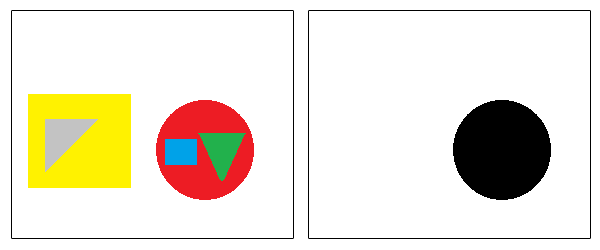
\includegraphics[scale=0.47]{graphics/threshold1.png}
		\caption{Ejemplo de filtrado threshold con umbral a 100}
		\label{fig:threshold1}
		\end{figure}
		
	Si, dado un caso similar en el que dos figuras estén superpuestas, pero que se comporten de forma distinta ante la aplicación del filtro (una se encuentra por debajo del umbral y otra por encima), entonces sí que se interpretará como dos figuras distintas (Figura~\ref{fig:threshold2}). Esto se produce debido a que, como se explica en la Sección~\ref{sec:deteccionContornos}, los contornos se buscan tanto en los perímetros externos de las figuras como en los internos.
	
		\begin{figure}[htbp]
		\centering
		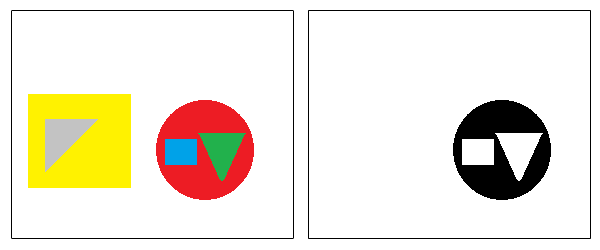
\includegraphics[scale=0.47]{graphics/threshold2.png}
		\caption{Ejemplo de filtrado threshold con umbral a 150}
		\label{fig:threshold2}
		\end{figure}
		
	Se trata de un algoritmo muy sencillo y rápido, pero en el que él éxito de los resultados depende tanto del umbral de entrada como de la imagen a analizar.
		
	\subsubsection{Adaptive Threshold}
	
	Se trata de una modificación del algoritmo anterior, donde el valor del umbral varía en cada región de la imagen. Este algoritmo también devuelve sólo una imagen binaria, pero aplica sobre ella un filtro más sofisticado que repara la mayor parte de los fallos del filtro anterior:

	\begin{center}
		$pixel(x,y) = \left\{
		\begin{array}{cc}
		MAXVAL 	& \text{ cuando } pixel(x,y) > T(x,y)\\ 
		0 	    & 	\text{e.o.c.}
		\end{array}\right.$
	\end{center}
	
	El umbral ya no es constante, sino que se convierte en el término $T(x,y)$ depende tanto de $x$ como de $y$. Existen muchas formas de calcular este término, pero en nuestro caso se calcula mediante la suma ponderada de los píxeles vecinos al $(x,y)$ dentro de un bloque de $3\times3$ píxeles donde el centro es el pixel a transformar. Tras haber realizado la suma, se le resta una constante c que en nuestro caso es 3.\\ \todo{Porqué 3 y porqué se le resta una constante si ya usas la media ponderada?}
	
	Con esta especificación, los resultados obtenidos son los mostrados en la Figura~\ref{fig:adaptive}. Como se puede observar, el resultado del filtro no depende de ningún valor y es más fiel que la mayoría de los resultados del threshold para figuras con este grado de simplicidad.\\
	
		\begin{figure}[htbp]
		\centering
		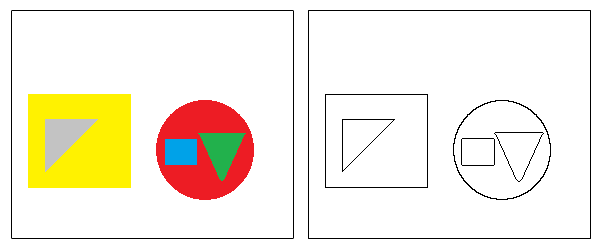
\includegraphics[scale=0.47]{graphics/adaptive.png}
		\caption{Ejemplo de filtrado adaptive}
		\label{fig:adaptive}
		\end{figure}
	
	\subsubsection{Canny}
	
	Usando como base el algoritmo de detección de bordes creado por John F. Canny en 1986 (cuya especificación se puede ver en \cite{pajares}), este filtro aborda el problema de la detección de figuras de una forma diferente: en vez de detectar el contenido de la figura, detecta el perímetro de las mismas.\\
	
	Usando el algoritmo de canny, que también devuelve una única imagen, se obtiene el resultado mostrado en la Figura~\ref{fig:canny}.\\
	
		\begin{figure}[htbp]
		\centering
		
\includegraphics[scale=0.47]{graphics/canny.png}
		\caption{Ejemplo de filtrado canny}
		\label{fig:canny}
		\end{figure}
		
	Esta nueva aproximación produce resultados satisfactorios, pero origina nuevos problemas: el perímetro detectado en el algoritmo puede no estar cerrado, provocando que la figura resultante no se represente de forma correcta en la estructura de salida.
	
	\subsubsection{Hue Division}
	
	Este algoritmo se basa en un concepto más simple: buscar manchas de color como agrupaciones de píxeles vecinos con colores ``parecidos''. Es decir, se dividen los tres canales de color en diferentes rangos, y se agrupan los píxeles contiguos cuyos valores de color caigan dentro de un mismo rango en todos los canales.\\
	
	Para establecer los rangos, se divide cada canal de color (rojo, verde y azul) en un número $n$ de intervalos. El parámetro $n$ es de entrada y común para los tres canales. De esta forma, se recorre la imagen por cada intervalo existente de colores, devolviendo las figuras encontradas en cada intervalo en imágenes de salida distintas.\\
	
	Por ejemplo, si $n$ es 3, quiere decir que por cada canal se establecerán 3 intervalos, en total cada color podrá caer dentro de uno de los $3*3*3=27$ intervalos. Por cada intervalo se devuelve una imagen con las figuras presentes en él, comprobando antes que no esté vacía (no existen figuras con colores dentro de ese intervalo). Se puede ver un ejemplo en la Figura~\ref{fig:huedivision}.
	
		\begin{figure}[htbp]
		\centering
		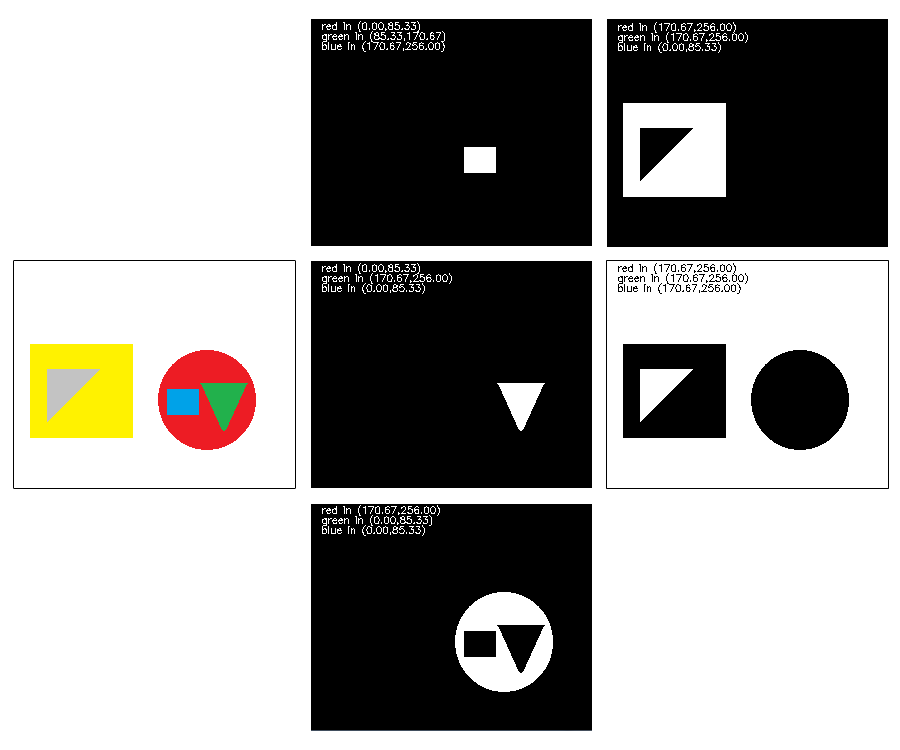
\includegraphics[scale=0.47]{graphics/huedivision.png}
		\caption{Ejemplo de filtrado hue division}
		\label{fig:huedivision}
		\end{figure}
	
	\subsubsection{Color Threshold}

	Se trata de una expansión del filtro Threshold para intentar resolver uno de sus principales problemas: dado que el filtro Threshold convierte la imagen en escala de grises para buscar píxeles que superen el umbral, puede darse el caso de que dos figuras con colores distintos se conviertan en el mismo tono de gris al convertirse a escala de grises. Este problema es independiente al método de transformación de RGB a escala de grises, e inherente al proceso en sí: al pasar de tres canales de color a un único canal, necesariamente varios valores de entrada van a coincidir en el mismo valor de salida (la función es sobreyectiva y el dominio de entrada es más grande que el de salida).\\
	
	Para resolver ese fallo, se realiza un filtro Threshold con tres umbrales distintos, uno para cada canal de color. Dado que estos umbrales van a poder ser manipulados por el usuario, se transformará previamente la imagen de RGB (rojo, verde y azul) a HSV (matiz, saturación y valor), que es un modelo más intuitivo para el ojo humano.\\
	
	Se pueden ver diferentes resultados de este filtro en las Figuras~\ref{fig:colorthres1} y ~\ref{fig:colorthres2}.
	
		\begin{figure}[htbp]
		\centering
		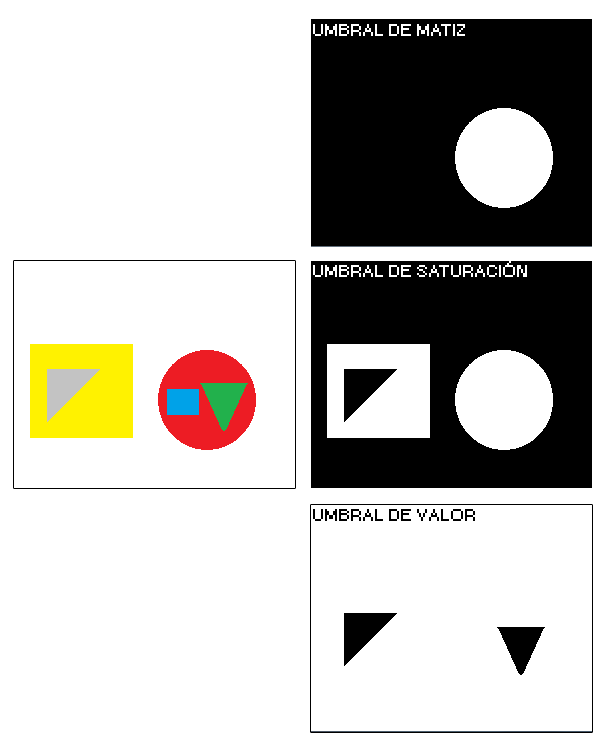
\includegraphics[scale=0.47]{graphics/colorthreshold.png}
		\caption{Ejemplo de filtrado color threshold: $Umbral_{H} = 55, Umbral_{S} = 150, Umbral_{V} = 205$}
		\label{fig:colorthres1}
		\end{figure}
	
		\begin{figure}[htbp]
		\centering
		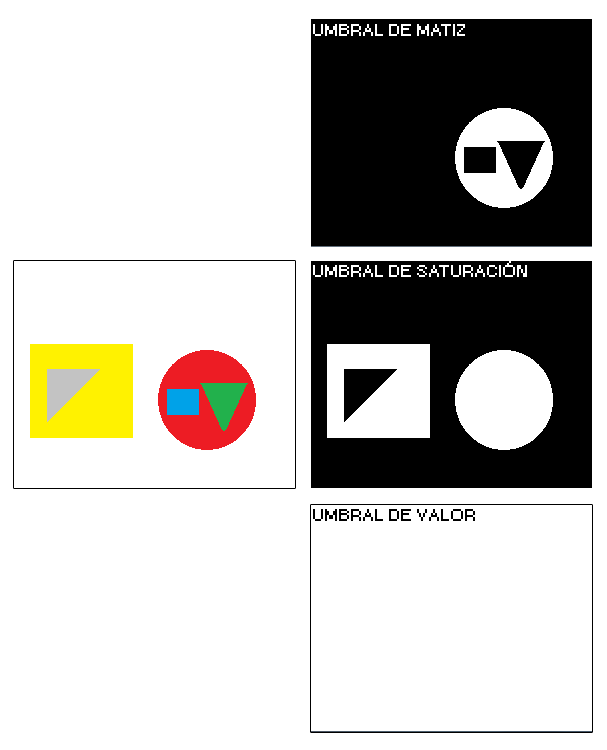
\includegraphics[scale=0.47]{graphics/colorthreshold2.png}
		\caption{Ejemplo de filtrado color threshold: $Umbral_{H} = 105, Umbral_{S} = 100, Umbral_{V} = 125$}
		\label{fig:colorthres2}
		\end{figure}
	
	
	
	\subsection{Detección de contornos y aproximación a polígonos}
	\label{sec:deteccionContornos}
	
	Una vez que tenemos la lista de imágenes binarias con las figuras localizadas, debemos proceder a representarlas en forma de polígonos. Para ello, primero detectaremos los contornos y posteriormente aproximaremos los mismos a polígonos.\\
	
	Para la primera parte (detección de contornos en base a una imagen binaria) haremos uso de la función \emph{cvFindContours} de OpenCV, cuyo resultado se puede ver en la Figura~\ref{fig:findcontours}.\\
	
		\begin{figure}[htbp]
		\centering
		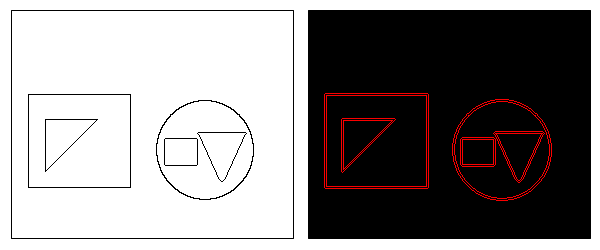
\includegraphics[scale=0.47]{graphics/contourdetection.png}
		\caption{Detección de contornos mediante OpenCV}
		\label{fig:findcontours}
		\end{figure}
		
	El ejemplo mostrado se ha basado en una imagen filtrada mediante el algoritmo Adaptive Threshold. Como se puede observar, una misma figura (el círculo) ha dado lugar a varios contornos. Este es un problema inherente a nuestro enfoque de detección de formas que se tratará más adelante.\\
	
	Posteriormente se usa otra función de OpenCV, \emph{cvApproxPoly}, para aproximar los contornos detectados a secuencias cerradas de vértices que podremos tratar con facilidad. El usuario puede decidir el grado de aproximación (de más simple a más fiel). Un ejemplo del resultado de esta función se ve en la Figura~\ref{fig:aproxpoly}\\
	
		\begin{figure}[htbp]
		\centering
		
\includegraphics[scale=0.47]{graphics/aproxpoly.png}
		\caption{Aproximación de polígonos mediante OpenCV}
		\label{fig:aproxpoly}
		\end{figure}
				
	Teniendo los polígonos listados, sólo resta organizar la información obtenida y guardarla en un archivo XML.\\
	
	Para ello se procede a calcular el área de cada polígono. Si es menor que la especificada como ruido por el usuario (ver Guía de Usuario, Capítulo~\ref{chap:guiauso}), entonces se desechará. Si no, se almacenará dentro de la estructura de figuras a archivar en XML. El color de cada polígono, por otro lado, se calculará haciendo la media del color de todos los píxeles que contiene.\\
	
	Para acabar, necesitamos organizar los polígonos resultantes en estructura de árbol, de forma que los polígonos que se encuentran dentro de otro polígono sean sus hijos en el árbol resultante. Es aquí donde surge el principal problema del análisis de imágenes: \textbf{los polígonos repetidos}.\\
	
	Como ya hemos comentado anteriormente, una misma mancha de color puede originar varios contornos, debido a que la figura se ha detectado dos veces en el proceso de filtrado (por ejemplo, si se encuentra dentro de dos umbrales en el filtro Color threshold) o a que el proceso de detección de contornos ha devuelto dos contornos similares a la figura dada, por particularidades internas del algoritmo de OpenCV.\\
	
	Esto va a originar que, irremediablemente, haya ocasiones en las que aparecerán varios contornos (y posteriormente polígonos) similares. Se procede pues, antes de continuar el análisis, a eliminar los polígonos repetidos. Para ello, se comprueba primero que tengan el mismo número de vértices y que los rectángulos mínimos que los contiene tengan área y posición similares. Una vez asegurado ese aspecto, se procede a calcular la siguiente condición:
	
	\begin{center}
		$sonSimilares(pol1,pol2,i,j) =$
	\end{center}
	\begin{center}
		
		$\left\{
		\begin{array}{ccc}
		cierto 	& \text{ si } & (dist(vertice(pol1,i), vertice(pol2,j)) < \epsilon)\wedge \forall k, 0 < k < N \\
				&             &  ((dist(vertice(pol1,(i + k) \%N), vertice(pol2,(j + k)\%N)) < \epsilon))\\
		 & & \\
		falso 	& 	          & \text{e.o.c.}
		\end{array}\right.$
		\end{center}
	
	para algún par de valores $i$ y $j$. $N$ es el número de vértices de ambos polígonos, $dist(p,q)$ es la función que calcula la distancia entre dos puntos del espacio bidimensional y $vertice(pol, i)$ devuelve el vértice $i$ de la lista de vertices del polígono $pol$. La constante $\epsilon$ determina lo cerca que deben estar los vértices entre sí par considerarse idénticos. \\
	
		\begin{figure}[htbp]
		\centering
		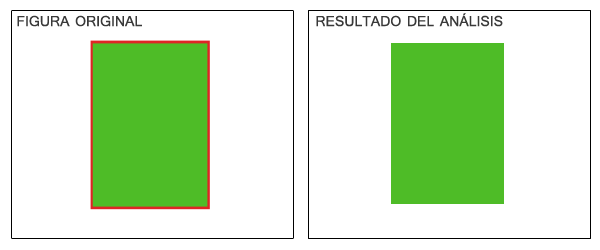
\includegraphics[scale=0.47]{graphics/reppoly.png}
		\caption{Caso de polígonos similares que no deben ser eliminados}
		\label{fig:colorsimilares}
		\end{figure}
	
	Sin embargo, puede darse el caso en que dos polígnos similares sean distintos y diferenciarse principalmente por el color (uno es la silueta del otro, ver Figura~\ref{fig:colorsimilares}. Dado que nunca trabajamos con el color, y éste se calcula \emph{a posteriori} (mirando los píxeles que contiene el polígono), no podremos saber de qué caso se trata \todo{esto suena raro}, ya que carecemos de la información necesaria debido a la naturaleza del proceso realizado. A pesar de todo, este caso es muy particular y no afecta al correcto desarrollo de la aplicación, por lo que no supone un problema en el análisis.\\
	
	Una vez eliminadas las figuras repetidas, se puede estructurar los polígonos en árboles, teniendo en cuenta que un polígono está dentro de otro cuando todos sus vértices están dentro de él. El rectángulo principal (que delimita el lienzo de la imagen) se elimina del análisis si ha sido detectado como polígono, ya que se encuentra en todas las imágenes y no aporta ninguna información relevante.\\
	
	El color calculado para cada polígono tenía en cuenta todos los píxeles que este contenía. Sin embargo, los polígonos que contienen otros polígonos han introducido información de más a la hora de calcular este color, ya que dentro de los polígonos que contienen se han tenido en cuenta los de sus hijos también. Es ahora que se conoce la estructura arbórea de la imagen cuando se pueden resolver estos detalles, recalculando el color de los polígonos que contienen a otros de forma que no se tenga en cuenta el color de sus polígonos internos.\\
	
	Finalmente, se guarda el contenido del análisis en un fichero XML, dando por terminado este proceso.
	


\section{Algoritmos de Composición}
\label{sec:algComposicion}
\todo{
esquema\\
\begin{itemize}
\renewcommand{\labelitemi}{\tiny$\blacksquare$}
\item intro a la composición: separado por voces.
\item cada voz: con cada compositor que lo haga
\item coletilla de final sin decidir todavía
\end{itemize}
}

Para componer la música separamos en diferentes voces. De tal modo que la unión de todas las voces da como resultado una pieza musical. En el estado actual del proyecto hemos identificado 4 voces diferentes dando un papel especial a cada una. Cada una de ellas son un proceso independiente aunque deben concordar en algunos aspectos para la correcta unión de todas ellos como por ejemplo la duración total. Todos los compositores de forma imprescindible reciben una figura, en la que se van a basar para componer, y una duración que será el tiempo que dura el trozo de música.

%----------------------------------------------------------------------------------------------------------------------------------------------------
\subsection{1ª Voz: Melodía Principal}

Normalmente en una composición suele haber una voz que destaca de la demás, que es la que el oído reconoce primero. Esta voz reproduce la melodía. Para poder crear la melodía, hemos separado el proceso en cuatro fases: procesar la figura, obtener duraciones, obtener tonos y sintetizar. 
La primera fase que consiste en procesar la figura de entrada. Sacamos sus vértices ordenados y seguidamente los lados con sus longitudes de forma que la figura se puede leer desde arriba en sentido horario (Figura~\ref{fig:Figura1Voz1}).

		\begin{figure}[htbp]
		\centering
		\hspace*{0.0in}
		
\includegraphics[scale=1.0]{graphics/simpletest1.png}
		\caption{Figura de entrada}
		\label{fig:Figura0Voz1}
		\end{figure}

		\begin{figure}[htbp]
		\centering
		\hspace*{0.0in}
		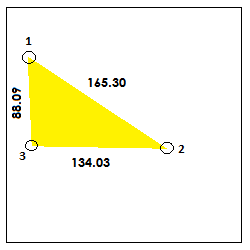
\includegraphics[scale=1.0]{graphics/simpletest1-F1.png}
		\caption{Figura de entrada con los vértices ordenados y con las longitudes de los lados}
		\label{fig:Figura1Voz1}
		\end{figure}

A continuación, en la segunda fase se calcula la longitud media de los lados y el lado más largo y más corto. Se asignan duraciones a cada lado teniendo en cuenta la duración máxima y la duración mínima con las longitudes recién calculadas (Figura~\ref{fig:Figura2Voz1}). Se usan las duraciones simples (figuras simples) de las notas en música obviando las compuestas (figuras compuestas), es decir, que se asignan duraciones de blancas, negras, corcheas, semicorcheas,... en vez de usar, por ejemplo, negra con doble puntillo que es una nota de duración negra más una corchea más una semicorchea. Buscar una equivalencia perfecta entre la longitud de los lados y la duración de las notas sería lo primero que pensaría el lector que podría ser la correspondencia más fiel, pero tras varias pruebas realizadas no se ha podido averiguar cómo hacerlo sin que se perdiera completamente el concepto de ritmo musical.

		\begin{figure}[htbp]
		\centering
		\hspace*{0.0in}
		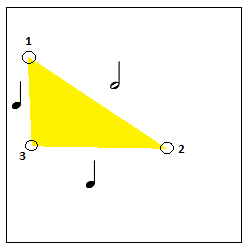
\includegraphics[scale=1.0]{graphics/simpletest1-F2.png}
		\caption{Figura de entrada con el ritmo producido}
		\label{fig:Figura2Voz1}
		\end{figure}

La tercera fase se centra en sacar los tonos de las notas que vamos a crear. Se tienen varias formas diferentes de conseguirlo que además se han llevado a cabo en diferentes trabajos (\cite{bricksConvertsMusic} \cite{ImageBaseComposition}). La aproximación usada se basa en la idea de estabilidad en la que se centra el trabajo de A. Pintado (\cite{portutesis}). Una figura es estable cuanto más suave sea su contorno, es decir, cuantos menos picos o irregularidades tenga. A. Pintado usa esta cualidad para generar ritmos a partir de figuras y líneas, nosotros lo vamos a usar para calcular tonos.

La obtención de los tonos viene de los ángulos de las figura, para ello se coge el primer vértice y se calcula su ángulo. Por ser la primera nota le asignamos el tono correspondiente al color de la figura dentro del sistema de colores usado (p. ej: Rojo en el sistema Scriabin es C "do"). A partir de ahí dependiendo de cuanto ha variado el ángulo del siguiente vértice respecto al anterior vamos asignando un tono más alto o más bajo (si sube o baja la diferencia de ángulo) (Figura~\ref{fig:Figura4Voz1}).

De forma experimental y tras varias pruebas, hemos obtenido una correspondencia entre la variación de ángulos y la cantidad de tonos que debe variar el nuevo tono respecto al anterior (Figura~\ref{fig:Figura3Voz1}). De este modo si la diferencia de ángulos es menor a 10º se sigue usando el mismo tono, si la diferencia está entre 10º y 30º se usa el tono vecino dentro de la escala, si está entre 30º y 120º el segundo tono más cercano del acorde, entre 120º y 240º el segundo tono más cercano del acorde y hasta 360º el tercer tono más cercano del acorde. Usamos el acorde fundamental con tono fundamental la nota del color de la figura para los grandes saltos porque conseguimos notas consonantes con el color de la figura. Este hecho se basa en la asociación que tiene Scriabin con los colores(``Referencia Aquí''), él hacía corresponder un color a un tono y su acorde fundamental sin distinguir entre acorde mayor o menor para cada una de las notas de la escala cromática.

		\begin{figure}[htbp]
		\centering
		\hspace*{0.0in}
		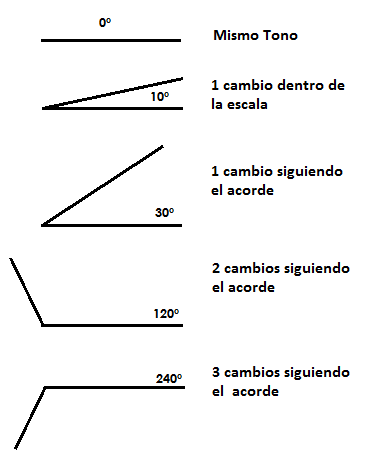
\includegraphics[scale=0.75]{graphics/tabla-corresp-Tono-Angulo.png}
		\caption{Tabla correspondencias entre ángulos y cambios de tono}
		\label{fig:Figura3Voz1}
		\end{figure}

De esta manera conseguimos que una figura simétrica con todos sus ángulos iguales suene la misma nota ya que su estabilidad es muy alta. El círculo sería la figura de mayor estabilidad y se correspondería a una nota de larga duración, pero por el proceso de análisis, el círculo se aproxima a un polígono regular de muchos lados y por tanto a muchas notas con el mismo tono.

		\begin{figure}[htbp]
		\centering
		\hspace*{0.0in}
		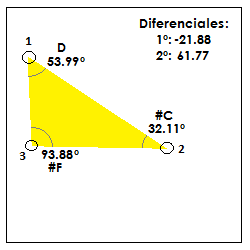
\includegraphics[scale=1.0]{graphics/simpletest1-F3.png}
		\caption{Figura de entrada con los ángulos y los tonos que produce}
		\label{fig:Figura4Voz1}
		\end{figure}

Por último, la cuarta fase que combina las duraciones con los tonos para crear las notas. Al final hemos obtenido un trozo de música de una de las voces.

Este algoritmo está implementado en la clase ComposerFigMelody2. Además hemos dejado otro compositor ComposerFigMelody que cambia la segunda y tercera fase, fruto de las primeras pruebas en la composición. En la segunda fase, al hacer corresponder las duraciones con las longitudes de los lados, se usan las duraciones compuestas con unidad mínima indivisible la semicorchea o unidades más pequeñas si la duración pedida del segmento de música es especial (no divisible en semicorcheas) (Figura~\ref{fig:Figura5Voz1}).

		\begin{figure}[htbp]
		\centering
		\hspace*{0.0in}
		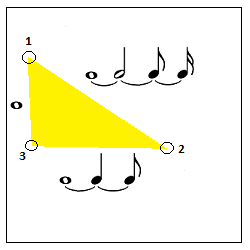
\includegraphics[scale=1]{graphics/simpletest1-F2_2.png}
		\caption{Figura de entrada con los lados y el ritmo conseguido}
		\label{fig:Figura5Voz1}
		\end{figure}

En la tercera fase, en vez de usar un algoritmo diferencial donde se tiene en cuenta la variación respecto al anterior ángulo examinado, se usa una correspondencia directa donde mayor águlo implica mayor salto de tono y el signo del ángulo es la dirección del salto (Figura~\ref{fig:Figura6Voz1}).

		\begin{figure}[htbp]
		\centering
		\hspace*{0.0in}
		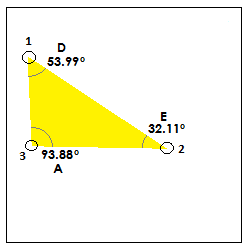
\includegraphics[scale=1]{graphics/simpletest1-F3_2.png}
		\caption{Figura de entrada con los ángulos y los tonos producidos}
		\label{fig:Figura6Voz1}
		\end{figure}

%----------------------------------------------------------------------------------------------------------------------------------------------------

\subsection{2ª Voz: Melodía Secundaria}

Para crear el acompañamiento o segunda voz, se usa la misma estructura que a la hora de componer la melodía principal aunque también necesitamos el segmento de melodía principal como entrada para poder componer sobre ella. 
La primera fase es igual que en la primera voz. La segunda fase también es igual salvo que al final introducimos un paso de adaptación. Debemos hacer una adaptación de la duración del total obtenido al analizar la figura (Figura~\ref{fig:Figura1Voz2}). Eso ocurre ya que se quiere que el segmento de música que se genera tenga una duración determinada normalmente menor a la melodía principal. Además se debe decidir en qué momento de la melodía principal se empieza a decorarla introduciendo la segunda voz.

 		\begin{figure}[htbp]
		\centering
		\hspace*{0.0in}
		
\includegraphics[scale=0.57]{graphics/todo.png}
		\caption{Figuras de entrada con los lados de la figura interior y las duraciones obtenidas}
		\label{fig:Figura1Voz2}
		\end{figure}

Esta función de adaptación se encarga de ir dividiendo a la mitad diferentes duraciones para reducir la duración total del segmento (o ir aumentando, duplicando duraciones, si se necesita aumentar la duración total). 

El otro cambio que hacemos es en la fase tercera. Mientras se generan los tonos se va analizando el comportamiento de la segunda voz respecto a la melodía principal. Este paso es necesario para disminuir las disonancias que puedan aparecer al juntar la primera y la segunda voz (Figura~\ref{fig:Figura2Voz2}). Por ello mientras se genera la nueva melodía se va haciendo pequeños cambios en la segunda voz que lleven a un resultado mejorado. Los cambios usados siguen los principios de las técnicas básicas contrapuntísticas. Estos cambios se activan cuando el intervalo entre la voz primera y la voz segunda es disonante y se mantiene un periodo alargado en el tiempo (igual o mayor a la duración media de las notas, normalmente una negra). Cómo se intenta minimizar los cambios, se suele hacer que si el cambio de tono era para subir, se sube menos o más el nuevo tono dependiendo de qué implica un menor cambio. Lo mismo cuando el cambio de tono es para bajar, se baja un poco más o menos el nuevo tono (Figura~\ref{fig:Figura3Voz2}).

		\begin{figure}[htbp]
		\centering
		\hspace*{0.0in}
		
\includegraphics[scale=0.57]{graphics/todo.png}
		\caption{Figuras de entrada con los ángulos y los tonos producidos sin técnicas contrapuntísticas}
		\label{fig:Figura2Voz2}
		\end{figure}

		\begin{figure}[htbp]
		\centering
		\hspace*{0.0in}
		
\includegraphics[scale=0.57]{graphics/todo.png}
		\caption{Figuras de entrada con los ángulos y los tonos producidos con técnicas contrapuntísticas}
		\label{fig:Figura3Voz2}
		\end{figure}

En la mayoría de ocasiones, la segunda voz se pide una duración menor que el segmento de primera voz que va acompañandolo, esto ocurre porque normalmente se pasa una figura de entrada menor que la usada para componer la melodía principal. Para que el segmento tenga la misma duración que el segmento de la primera voz se rellenan los huecos (delante y/o detrás) del trozo de música compuesto con silencios.

%----------------------------------------------------------------------------------------------------------------------------------------------------

\subsection{3ª Voz: Bajo}

Para el bajo, se ha cogido un algortimo simple que consiste en notas de duración dada (por defecto redondas) que tengan como tono el color de la figura de entrada y que rellene la duración completa dada (Figura~\ref{fig:Figura1Voz3}).

		\begin{figure}[htbp]
		\centering
		\hspace*{0.0in}
		
\includegraphics[scale=0.57]{graphics/todo.png}
		\caption{Figura de entrada con los lados y los tonos producidos}
		\label{fig:Figura1Voz3}
		\end{figure}

Otra posibilidad habilitada para el bajo es usar la algoritmia de la primera voz pero transportandola una o varias octavas más abajo (Figura~\ref{fig:Figura2Voz3}). El número de octavas depende del tono más agudo y el tono más grave que hay en la melodía compuesta. Si se tiene que al transportar la melodía dos octavas más grave se sale del límite de representación de las notas, entonces sólo se hace más grave una octava.

		\begin{figure}[htbp]
		\centering
		\hspace*{0.0in}
		
\includegraphics[scale=0.57]{graphics/todo.png}
		\caption{Figura de entrada con los lados y los tonos producidos}
		\label{fig:Figura2Voz3}
		\end{figure}

%----------------------------------------------------------------------------------------------------------------------------------------------------

\subsection{4ª Voz: Ritmo}

Para el ritmo se creó una primera versión basada en la disposición de los vértices. Se dividía la figura en varias secciones de ángulos dejando cada vértice dentro de una sección. Estas secciones son configurables para hacerlas en distintas proporciones. Una vez se tienen los vértices de cada sección, se sustituyen por ritmos. De tal modo que si no hay un vértice en una sección, esta tiene un silencio y si hay un vértice, entonces hay un pulso de ritmo (Figura~\ref{fig:Figura1Voz4}). Este ritmo se repite durante la duración dada por entrada.

		\begin{figure}[htbp]
		\centering
		\hspace*{0.0in}
		
\includegraphics[scale=0.57]{graphics/todo.png}
		\caption{Figura de entrada y los ritmos producidos}
		\label{fig:Figur1Voz4}
		\end{figure}

El otro ritmo implementado se basa en el concepto de inestabilidad de una figura de A. Pintado (\cite{portutesis}). Por defecto creamos un ritmo que consiste en pulsos largos (la duración de estos pulsos se pueden configurar). A cada nota le es asignado una serie de vértices dependiendo de la densidad de vértices de la figura. Después se va calculando cuanto de desviación se produce en esos vértices respecto al círculo de área igual a la figura y con centro el punto de equilibrio de la figura (Figura~\ref{fig:Figura2Voz4}). A mayor desviación, mayor inestabilidad luego el ritmo se subdivide en más notas y de menor duración (Figura~\ref{fig:Figura3Voz4}).

		\begin{figure}[htbp]
		\centering
		\hspace*{0.0in}
		
\includegraphics[scale=0.57]{graphics/todo.png}
		\caption{Figura de entrada y el círculo equivalente}
		\label{fig:Figura2Voz4}
		\end{figure}

		\begin{figure}[htbp]
		\centering
		\hspace*{0.0in}
		
\includegraphics[scale=0.57]{graphics/todo.png}
		\caption{Figura de entrada y los ritmos producidos}
		\label{fig:Figura3Voz4}
		\end{figure}

%----------------------------------------------------------------------------------------------------------------------------------------------------

\subsection{Mixer}

Los anteriores algoritmos son para crear un trozo de musica de una voz a partir de una figura, pero tenemos que saber en qué momento vamos a llamar a cada algoritmo y con qué figuras. Para ello está el Mixer.

En una primera implementación el mixer se encargaba de ordenar las figuras en orden de relevancia siguiendo el parámetro de vistosidad calculado a partir de tres características de la figura.
La primera es lo vistosidad del color de la figura. Para ello descomponemos el color en sus tres componentes principales RGB y damos peso a cada uno de ellos y lo multiplicamos por la saturación del color.
La segunda componente es el área que ocupa la figura. Cuanto más grande sea, más vistosa es.
La tercera componente es la distancia que tiene del centro de la imagen. El ojo humano enfoca de centro a laterales cuando ve una imagen por primera vez, por ello tiene más vistosidad una figura que se encuentra en el centro de la imagen que en un lateral.

	\begin{center}
		$vistosidad(Figura) =$
	\end{center}
	\begin{center}
		
		$\left\{
		\begin{array}{cc}
		A = 0.5f; B = 0.3f; C = 0.2f;\\ 
		pR = 0.45f; pG = 0.35f; pB = 0.20f;\\
		A*getSaturation()*(rgb.r*pR + rgb.g*pG + rgb.b*pB)\\
		 + B*area + C*distanceCenter
		\end{array}\right.$
	\end{center}

Tras haber ordenado las figuras por vistosidad vamos componiendo con cada una de forma iterativa las distintas voces. En el primer mixer que hicimos, sólo se componía  de melodía y ritmo. Para la segunda versión del mixer se sigue calculando la vistosidad como se explicó pero en vez de ordenar todas las figuras, ordenamos solo las figuras que están en la imagen sin estar dentro de otra figura, las llamadas figuras padre. Una vez las tenemos vamos iterando por cada figura padre componiendo su melodía, bajo y ritmo. Si la figura padre tiene otras figuras dentro de ella (figuras hijas), entonces también se añade la segunda melodía dando como entrada al algoritmo de composición de acompañamiento esta segunda figura (la figura hija). Por cada figura interior se compone un nuevo bloque de la figura padre con diferentes acompañamientos (Figura~\ref{fig:Figura1Mixer}).

		\begin{figure}[htbp]
		\centering
		\hspace*{0.0in}
		
\includegraphics[scale=0.57]{graphics/todo.png}
		\caption{Figuras de entrada las voces producidas}
		\label{fig:Figura1Mixer}
		\end{figure}

Una vez tenemos compuestas todas las voces, es el mixer el que se encarga de juntarlas y llamar a la creación de la partitura y posterior conversión a midi.


























